\subsection{Serviço Anti-Spam -- Spamassassin}

O serviço de detecção de \emph{spam}\footnote{Spam é uma mensagem electrónica
não-solicitada enviada em grande escala.} utilizado no servidor é o
\emph{Spamassassin}.

O ficheiro de configuração deste serviço é:

\begin{Verbatim}[commandchars=\\\{\}]
/etc/mail/spamassassin/local.cf
\end{Verbatim}

O existem vários comandos para controlar este serviço:

\ServiceCommands{spamassassin}

O serviço anti-spam também poderá ser gerido utilizando a interface web disponibilidada para o efeito. Para tal, deverá aceder à secção Servers->SpamAssassin Mail Filter na árvore de acessos do lado esquerdo. Posteriormente deverá encontrar uma página semelhante à seguinte:

\begin{figure}[H]
    \begin{center}
        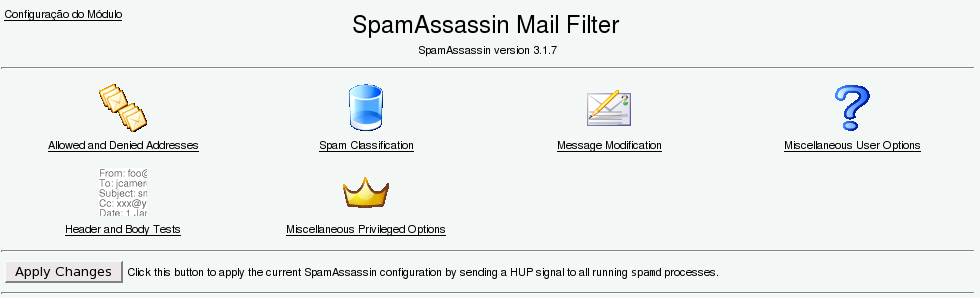
\includegraphics[width=10cm]{include/img/spam1}
    \end{center}
    \caption{Configuração do SpamAssassin}
    \label{fig:SPAM1}
\end{figure}

Relembramos que o mecanismo anti-spam apenas marca o correio electrónico como possível de ser spam. É no entanto possível excluír determinados endereços e/ou domínios de email desta marcação (o que denominamos de whitelist) e marcar outros endereços e/ou domínios como spam (o que denominamos blacklist ou lista-negra). Para que possa gerir estas listas, deverá escolher a opção "Allowed and Denied Addresses" e deverá encontrar uma página semelhante à seguinte:

\begin{figure}[H]
    \begin{center}
        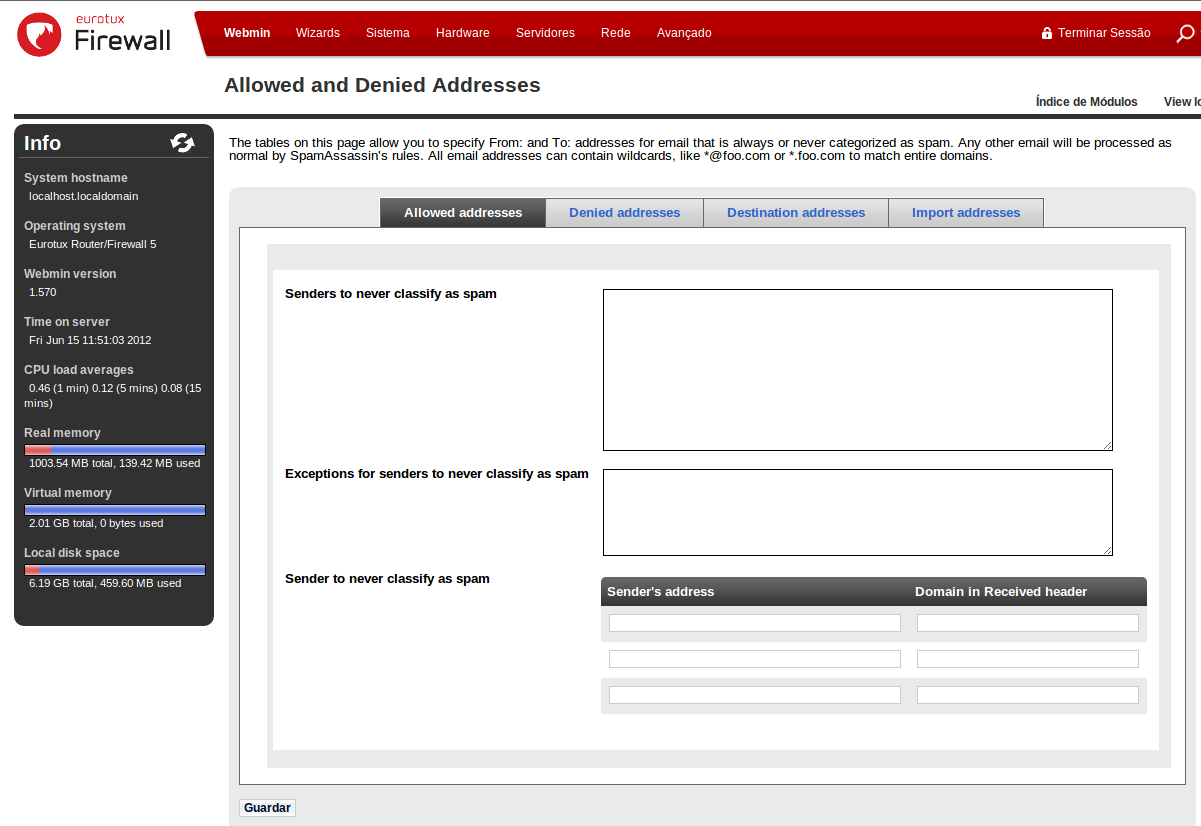
\includegraphics[width=10cm]{include/img/spam2}
    \end{center}
    \caption{Whitelist e blacklist}
    \label{fig:SPAM2}
\end{figure}

Para adicionar endereços à whitelist deverá preencher a caixa intitulada "From: addresses to never classify as spam". Deste modo todos os emails cujo rementente estiver nesta lista não serão marcados como correio não solicitado vulgo spam. A título exemplificativo, se adicionássemos *.eurotux.com nesta caixa, todo o correio cujo rementente é da eurotux não será marcado como spam.

Para adicionar endereços à blacklist deverá preencher a caixa intitulada "From: addresses to always classify as spam". O modelo de funcionamento é análogo à whitelist.
Posteriormente a qualquer alteração deverá carregar no botão "Guardar" para gravar as alterações.

A marcação de spam é efectuada utilizando heurísticas que pontuam determinados padrões. Quando essa pontuação atinge um determinado valor o email é considerado spam e marcado de acordo. Este limite de pontuação poderá ser modificado. Para tal deverá utilizar o icon "Spam Classification" no ecrã de configuração do spamassassin.

\begin{figure}[H]
    \begin{center}
        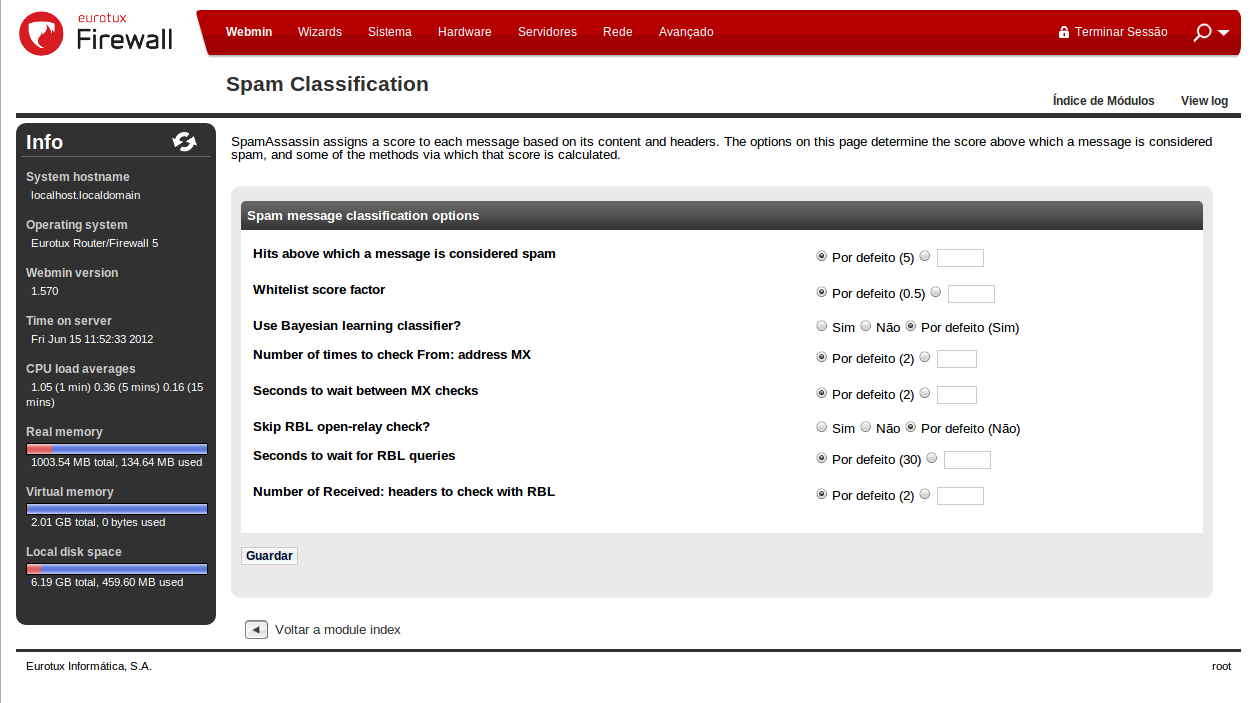
\includegraphics[width=10cm]{include/img/spam3}
    \end{center}
    \caption{Nível de spam}
    \label{fig:SPAM3}
\end{figure}

No primeiro item ("Hits above which a message is considered spam") é definido o valor a partir do qual o email é considerado spam. O valor por omissão é 5 pontos.
